\chapter{Thermodynamics and Finite Size Scaling}

	In this Chapter,  a comparison between mean and exact thermodynamic variables is presented along with the estimation of the Curie temperature for the infinite lattice.

	Firstly one important note on thermodynamic calculations. Extracting thermodynamic information from the JDoS can be a difficult process, specially when trying to study large systems. Although the formulas from Chapter 1 are easy to understand, the problem arrives when trying to actually compute the partition function and consequent Boltzmann factors for the ensemble average variables. 
	
	For large systems, the values from the JDoS are very large, for instance, for an L16 SS Ising system, some of the values of the JDoS are of the order $10^{74}$. We can not keep summing and multiplying these values to compute $Z$, since we run into overflow errors. For low temperatures we run into the same error, since the exponential gets very large. Instead we have to work with the logarithms of these functions to extract the thermodynamics out of the JDoS. We can use the following observation,
\begin{equation}
	\ln \left[  \sum_i a_i \right] = \ln(a_0) + \ln\left[ 1 + \sum_{i \neq 0} \frac{a_i}{a_0} \right]
\end{equation}

\section{Mean and Exact Thermodynamic Variables}

	As previously mentioned in Chapter 1, we can calculate thermodynamic variables from the JDoS in two different ways. One by using the ensemble averages through the partition function and Boltzmann factor and another by using the minimum of the Helmholtz free energy. For three different square lattice system sizes, these thermodynamic quantities can be seen in Figure \ref{thermo_4}. For the $C_{minF}$, there is only one size since smaller sizes give very inaccurate results due to numerical differentiation, Equation \ref{C_min}.
	
	We would expect that the thermodynamic quantities computed by these two equivalent ways would yield similar results. By a quick analysis of Figure \ref{mod_M} and \ref{M} we can see that the magnetization curves computed by the two methods are not that similar. The $\langle |M| \rangle$ has a flatter curve while the $M_{minF}$ has a more pronounced curve, where you can better see the phase transition. If we kept increasing the number of spin particles in our simulations, eventually these two ways would give us very similar results, and, for the infinite lattice, they would be equivalent and equal to the Onsager solution. 
\begin{figure}[h]
	\centering
	\subfigure[]{
		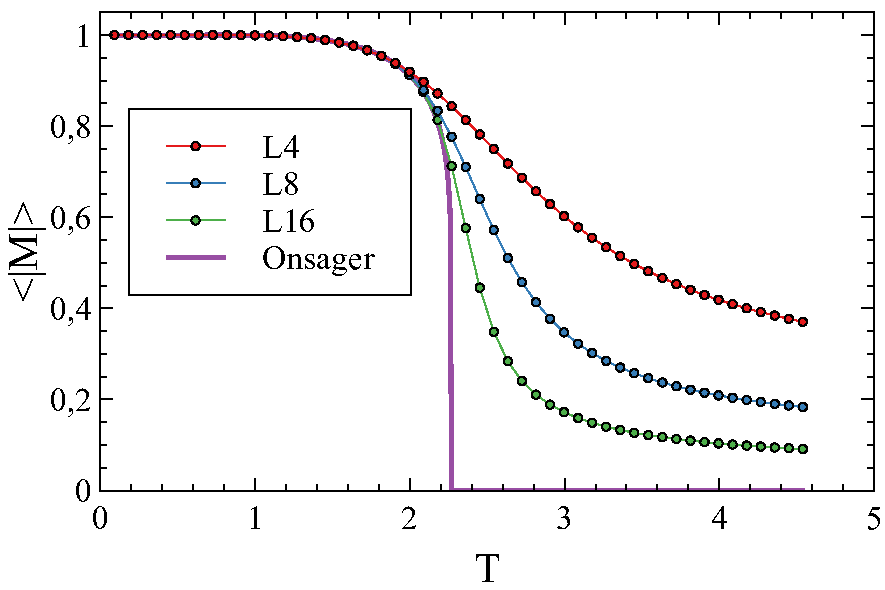
\includegraphics[scale=0.48]{thermodynamics/thermodynamics_finite_size_03.pdf}
		\label{mod_M}
	}	
	\subfigure[]{
		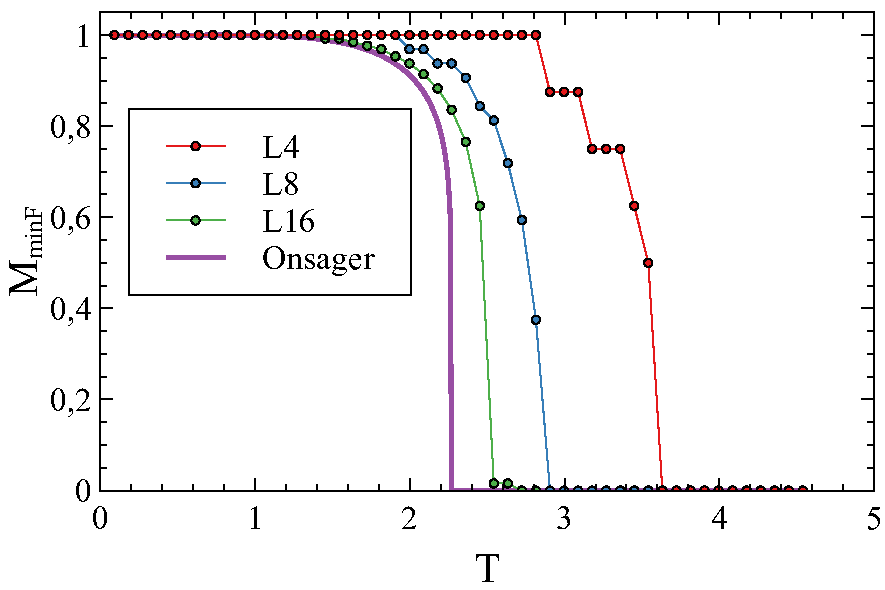
\includegraphics[scale=0.48]{thermodynamics/thermodynamics_finite_size_02.pdf}
		\label{M}
	}	
	
	\subfigure[]{
		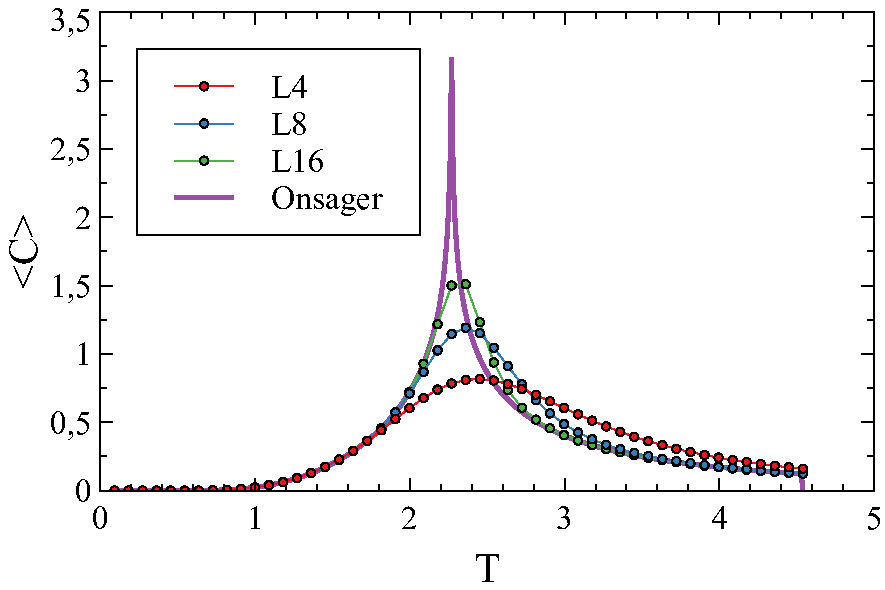
\includegraphics[scale=0.48]{thermodynamics/thermodynamics_finite_size_05.pdf}
		\label{mean_C}
	}	
	\subfigure[]{
		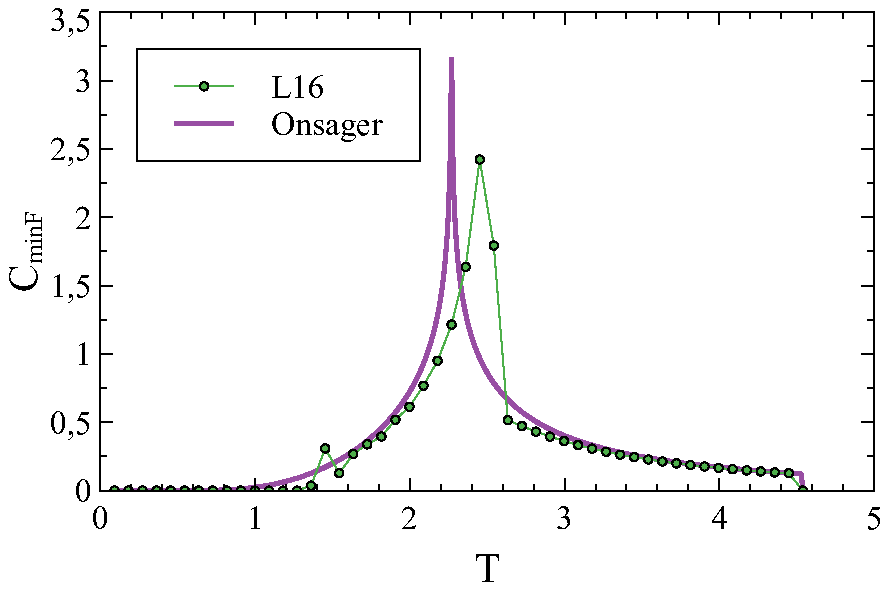
\includegraphics[scale=0.48]{thermodynamics/thermodynamics_finite_size_04.pdf}
		\label{C}
	}
	\caption{Thermodynamics for 3 different lattice sizes compared with the exact solution by Onsager. (a) $\langle |M| \rangle$. (b) $M_{minF}$. (c) $\langle C \rangle$. (d) $C_{minF}$.}
	\label{thermo_4}
\end{figure}
	Another noteworthy aspect is the Curie temperature $T_C$ that we can extract from these two curves. The point in which a phase transition occurs is the inflexion point, therefore the point where the first derivative has a relative extrema. In Table \ref{TC_table} there can be seen the Curie temperatures estimated through the two magnetization curves for the different system sizes. 

\begin{table}[h]
\centering
\caption{Curie temperature estimated by the $\langle |M| \rangle$ and $M_{minF}$ for the three different lattice sizes and their respective error. The first derivative of the magnetization has a curve with a shape of a Gaussian function. Thus the error can be estimated considering the half height width.}
\begin{tabular}{c|ccc|ccc}
L  & $T_C\ \langle |M| \rangle$ & $\Delta -$ & $\Delta +$ & $T_C\ M_{minF}$ & $\Delta -$ & $\Delta +$ \\ \hline
4  & 2.542                                                 & 0.726                  & 0.908         & 3.541           & 0.091                  & 0.091                \\
8  & 2.452                                                 & 0.454                   & 0.363                  & 2.815           & 0.182         & 0.091                  \\
16 & 2.361                                                 & 0.272                  & 0.182                  & 2.452           & 0.091                  & 0.091                 
\end{tabular}
\label{TC_table}
\end{table}

	The Curie temperatures taken from the average and exact thermodynamic variables are much different. The $T_C \langle |M| \rangle$ is closer to the $T_C$ for the infinite lattice but $T_C\ M_{minF}$ has much less statistical error thus it is a more precise value, since the magnetization curve is more pronounced.
	
	The mean specific heat and the specific heat obtained from the minimum of $F$, Figure \ref{mean_C} and \ref{C},respectively, have similar properties as the magnetization. The mean heat capacity has a smoother curve compared to the Onsager solution while the exact specific heat has a curve similar to the Onsager solution where the phase transition and Curie temperature are more pronounced.

\pagebreak

\section{Estimating $T_C$ for the Infinite Lattice}

	The estimation the Curie temperate for the infinite system can be obtained by two different methods \cite{Landau_Book}. The first method relies on knowing the Curie temperature for each $L$ for example the peak on the heap capacity of by the differentiation of the magnetization. This $T_C(L)$ defines a phase transition in the finite lattice. Thus we can use the linear relation
\begin{equation}\label{TC_reg_exp}
	T_C(L) = T_C(\infty) + cL^{-1/\nu},
\end{equation}
where $\nu$ is equal to unity to consider the Onsager solution, $T_C\approx2.269$ \cite{Onsager1944}.
Another way is to use the fourth order cumulant $U_L$, known as the Binder cumulant, defined as
\begin{equation}
	U_L(T) = 1 - \frac{\langle M^4 \rangle}{3\langle M^2 \rangle^2}.
\end{equation}
For a infinite system size, $L\rightarrow\infty$, the cumulant takes a value of 0 for $T>T_C$ and $2/3$ for $T<T_C$.
Plotting the Binder cumulant for different system sizes, the curves all cross a point. The temperature of this point is an estimation of the Curie temperature for the infinite lattice. The accuracy of these two methods greatly improves if larger system sizes are considered.

\begin{figure}[h]
	\centering
	\subfigure[]{
		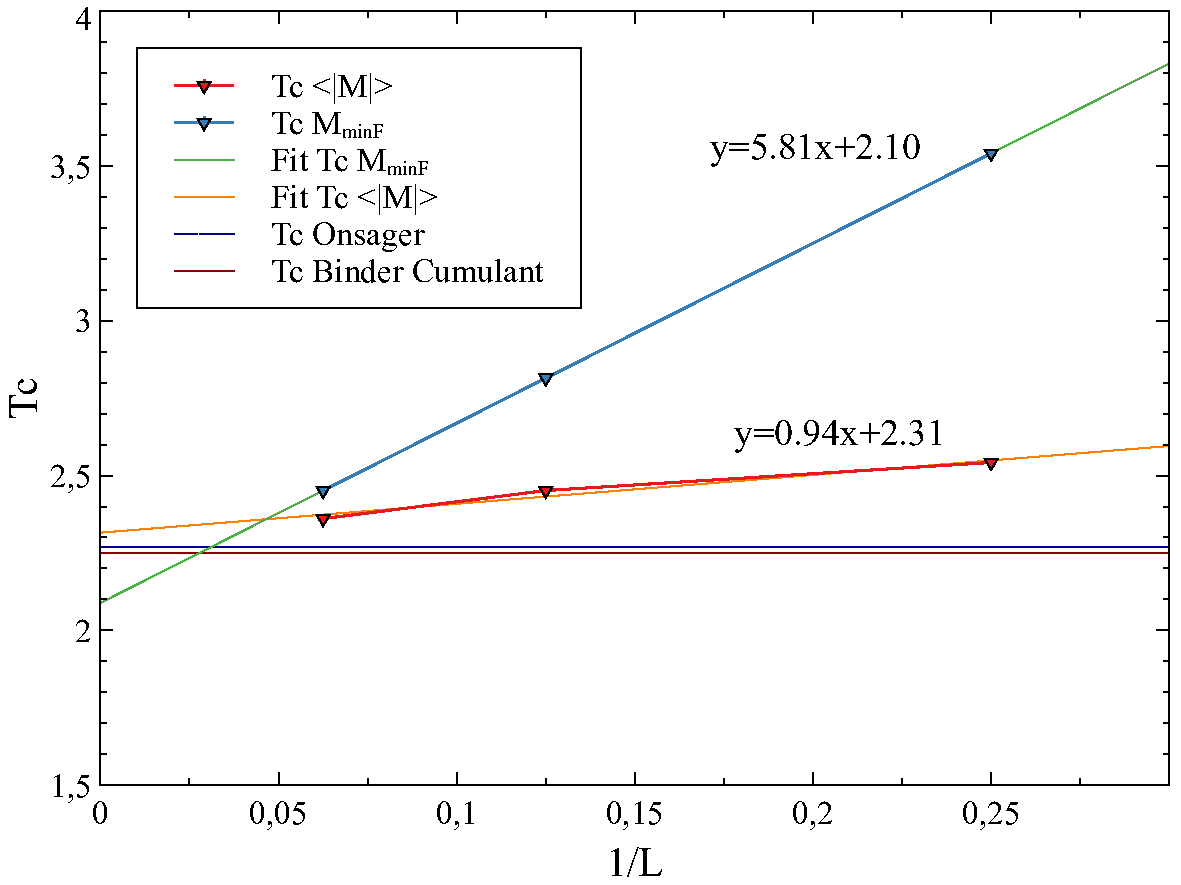
\includegraphics[scale=0.37]{thermodynamics/thermodynamics_finite_size_01.pdf}
		\label{TC_reg}
	}	
	\subfigure[]{
		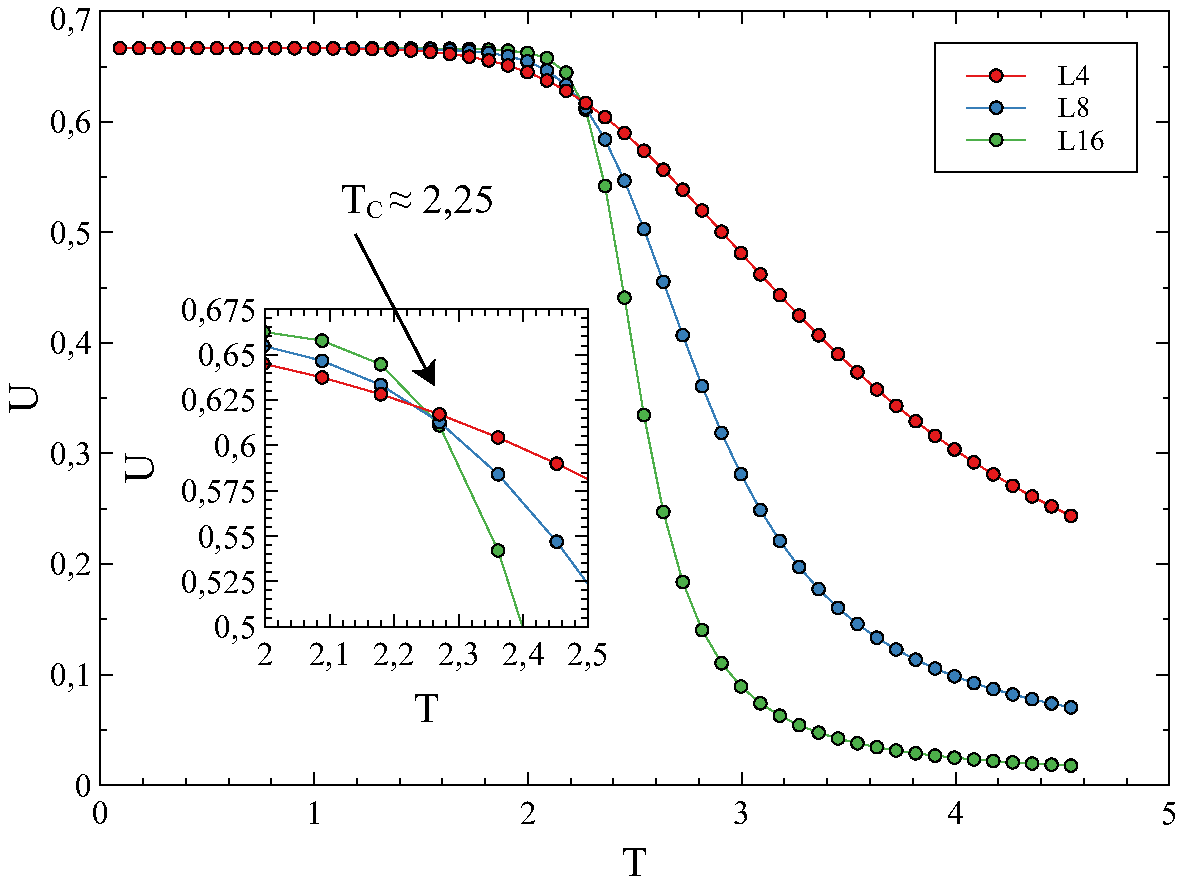
\includegraphics[scale=0.37]{thermodynamics/thermodynamics_finite_size_08.pdf}
		\label{binder}
	}
	\caption{(a) Linear regression of the $T_C(L)$ from $\langle |M| \rangle$ and $M_{minF}$ as function of $1/L$. (b) Binder cumulant for different system sizes.}
	\label{TC_inf}
\end{figure}

	For the first method, a linear regression with the $T_C(L)$ values from Table \ref{TC_table} for the two magnetization curves is presented in Figure \ref{TC_reg}. As we are only interest in the $T_C(\infty)$ from Equation \ref{TC_reg_exp}, for the the $\langle |M| \rangle$ curve the estimated critical temperature for the infinite lattice is approximately $2.31$ while for the $M_{minF}$ is approximately $2.10$. 
	For the second method, the Binder cumulant for different L values is displayed in Figure \ref{binder}. The critical point is the point in which the curves intersect each other. This yields an estimation $T_C \approx 2.25$.
	
	For the available system sizes, the Binder cumulant gave the best results with $T_C \approx 2.25$. This is a great method of estimating the $T_C$ for the infinite lattice when we do not have results from bigger lattices, L32 or L64. The critical temperatures estimated from linear fitting the $T_C$ values form magnetizations is a good method to estimate the $T_C$ for the infinite if we have a JDoS for a bigger system.All of these estimation could be improved by considering larger systems, for example the L32 simple square.








